
\usetikzlibrary{arrows}

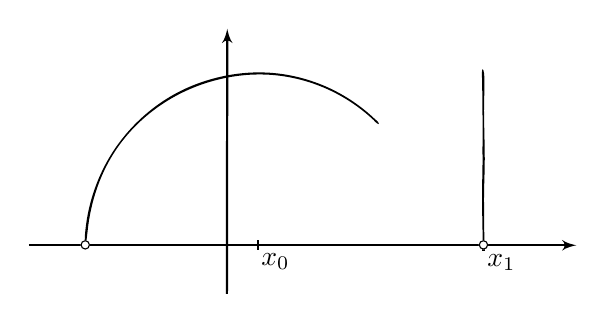
\begin{tikzpicture}[y=0.80pt, x=0.8pt,yscale=-1,scale=0.3, inner sep=0pt, outer sep=0pt]
\begin{scope}[shift={(220.0315,-356.64289)}]% layer1
  \begin{scope}[shift={(3147.7678,-1427.0496)}]% g1988
    % path2584-0-9
    \path[draw=black,line join=miter,line cap=butt,line width=0.800pt,-latex']
      (-3367.7993,2109.6489) -- (-2543.3619,2109.6489);

    % path2582-4-4
    \path[draw=black,line join=miter,line cap=butt,line width=0.800pt,-latex']
      (-3069.5306,2182.6982) -- (-3068.9608,1783.6932);

  \end{scope}
  
  \path[cm={{1.0,0.0,0.0,-1.0,(3140.5045,2591.4389)}},color=black,fill=black,line
    width=0.800pt] (-3275.9219,1924.7961) .. controls (-3274.0064,1949.1681) and
    (-3268.7857,1973.2307) .. (-3260.4507,1996.1851) .. controls
    (-3252.1157,2019.1395) and (-3240.6585,2040.9822) .. (-3226.3161,2060.7308) ..
    controls (-3218.1656,2071.9535) and (-3209.1713,2082.5585) ..
    (-3199.3587,2092.3795) .. controls (-3187.1384,2104.6086) and
    (-3173.7246,2115.6571) .. (-3159.3392,2125.2681) .. controls
    (-3144.9538,2134.8790) and (-3129.5957,2143.0509) .. (-3113.5346,2149.5012) ..
    controls (-3113.5346,2149.5012) and (-3113.5346,2149.5012) ..
    (-3113.5346,2149.5012) .. controls (-3113.1699,2149.6476) and
    (-3112.8048,2149.7932) .. (-3112.4394,2149.9379) .. controls
    (-3097.0993,2156.0119) and (-3081.2310,2160.7397) .. (-3065.0449,2163.9877) ..
    controls (-3048.8588,2167.2358) and (-3032.3546,2169.0015) ..
    (-3015.8188,2169.1274) .. controls (-2999.8796,2169.2486) and
    (-2983.9164,2167.8441) .. (-2968.2563,2164.8673) .. controls
    (-2951.0237,2161.5916) and (-2934.1341,2156.5782) .. (-2917.9460,2149.8888) ..
    controls (-2888.8995,2137.8841) and (-2862.1914,2120.4577) ..
    (-2839.4920,2098.9265) .. controls (-2836.8258,2096.8474) and
    (-2835.1135,2095.0508) .. (-2834.1618,2093.7239) .. controls
    (-2833.2100,2092.3970) and (-2833.0168,2091.5377) .. (-2833.3988,2091.2677) ..
    controls (-2833.7809,2090.9978) and (-2834.7367,2091.3147) ..
    (-2836.1176,2092.3096) .. controls (-2837.4985,2093.3041) and
    (-2839.3032,2094.9740) .. (-2841.4364,2097.4050) .. controls
    (-2863.9308,2118.5347) and (-2890.3362,2135.6017) .. (-2918.9853,2147.3259) ..
    controls (-2934.7322,2153.7707) and (-2951.1412,2158.6130) ..
    (-2967.8722,2161.7989) .. controls (-2983.6622,2164.8057) and
    (-2999.7601,2166.1917) .. (-3015.8188,2166.0130) .. controls
    (-3031.7764,2165.8355) and (-3047.6958,2164.1152) .. (-3063.3128,2161.0052) ..
    controls (-3078.9298,2157.8952) and (-3094.2448,2153.3978) ..
    (-3109.0654,2147.6431) .. controls (-3110.1330,2147.2286) and
    (-3111.2004,2146.8062) .. (-3112.2672,2146.3759) .. controls
    (-3127.6217,2140.1844) and (-3142.8538,2132.3217) .. (-3157.2876,2122.9313) ..
    controls (-3171.7213,2113.5409) and (-3185.3479,2102.6268) ..
    (-3197.5901,2090.6108) .. controls (-3207.7492,2080.6412) and
    (-3216.9054,2069.8903) .. (-3224.9220,2058.7675) .. controls
    (-3231.9232,2049.0535) and (-3237.9985,2039.0203) .. (-3243.2902,2028.7549) ..
    controls (-3248.5820,2018.4895) and (-3253.0914,2007.9901) ..
    (-3256.9204,1997.2658) .. controls (-3260.7494,1986.5415) and
    (-3263.8991,1975.5911) .. (-3266.4128,1964.3674) .. controls
    (-3268.9264,1953.1438) and (-3270.8056,1941.6460) .. (-3272.0133,1929.7871) ..
    controls (-3272.2533,1927.6235) and (-3272.5773,1924.8845) ..
    (-3272.9079,1922.1027) .. controls (-3273.2386,1919.3208) and
    (-3273.5755,1916.4957) .. (-3273.9090,1914.1696) .. controls
    (-3274.2424,1911.8435) and (-3274.5767,1910.0163) .. (-3274.9407,1909.2419) ..
    controls (-3275.3047,1908.4675) and (-3275.7077,1908.7460) ..
    (-3276.1132,1910.6445) .. controls (-3276.5112,1914.8042) and
    (-3276.2471,1920.1155) .. (-3275.9219,1924.7961) -- cycle;
\filldraw[white](-135,682) circle (5pt);
  \draw(-135,682) circle (5pt);
  % path2032
  \path[draw=black,line join=miter,line cap=butt,line width=0.800pt]
    (124.5441,675.1125) -- (124.5441,689.1781);

  % text2036
  \path[fill=black] (130.17809,718.74866) node[above right] (text2036) {$x_0$};

  \begin{scope}[shift={(2906.3668,-1422.8206)}]% g1992
  \end{scope}
  % path2040
  \path[fill=black] (462.1640,424.4330) .. controls (462.8869,445.4724) and
    (462.7591,466.5429) .. (463.0949,487.6326) .. controls (463.4306,508.7221) and
    (462.9294,529.8297) .. (463.1058,550.9405) .. controls (463.2821,572.0514) and
    (462.1360,593.1655) .. (462.3806,614.2687) .. controls (462.6252,635.3717) and
    (462.9609,656.4639) .. (463.5014,677.5303) .. controls (462.3453,683.3565) and
    (467.2841,682.9759) .. (465.9389,677.3598) .. controls (465.5684,656.4858) and
    (465.4085,635.5856) .. (465.3263,614.6761) .. controls (465.2441,593.7667) and
    (466.5393,572.8483) .. (466.4796,551.9380) .. controls (466.4199,531.0278) and
    (465.6750,508.1669) .. (465.3719,487.2905) .. controls (465.0687,466.4141) and
    (466.5077,447.5234) .. (465.6953,426.7155) .. controls (465.4684,422.9163) and
    (464.1545,415.0762) .. (462.4766,418.3411) .. controls (462.0479,420.1309) and
    (462.1372,422.4139) .. (462.1640,424.4330) -- cycle;
  % path2032-8
  \path[draw=black,line join=miter,line cap=butt,line width=0.800pt]
    (464.6885,677.6608) -- (464.6885,691.7264);
\filldraw[white](464.5,682) circle (5pt);
  \draw(464.5,682) circle (5pt);

  % text2036-5
  \path[fill=black] (470.32239,721.29706) node[above right] (text2036-5) {$x_1$};

\end{scope}

\end{tikzpicture}

